\begin{figure*}[t]
\centering
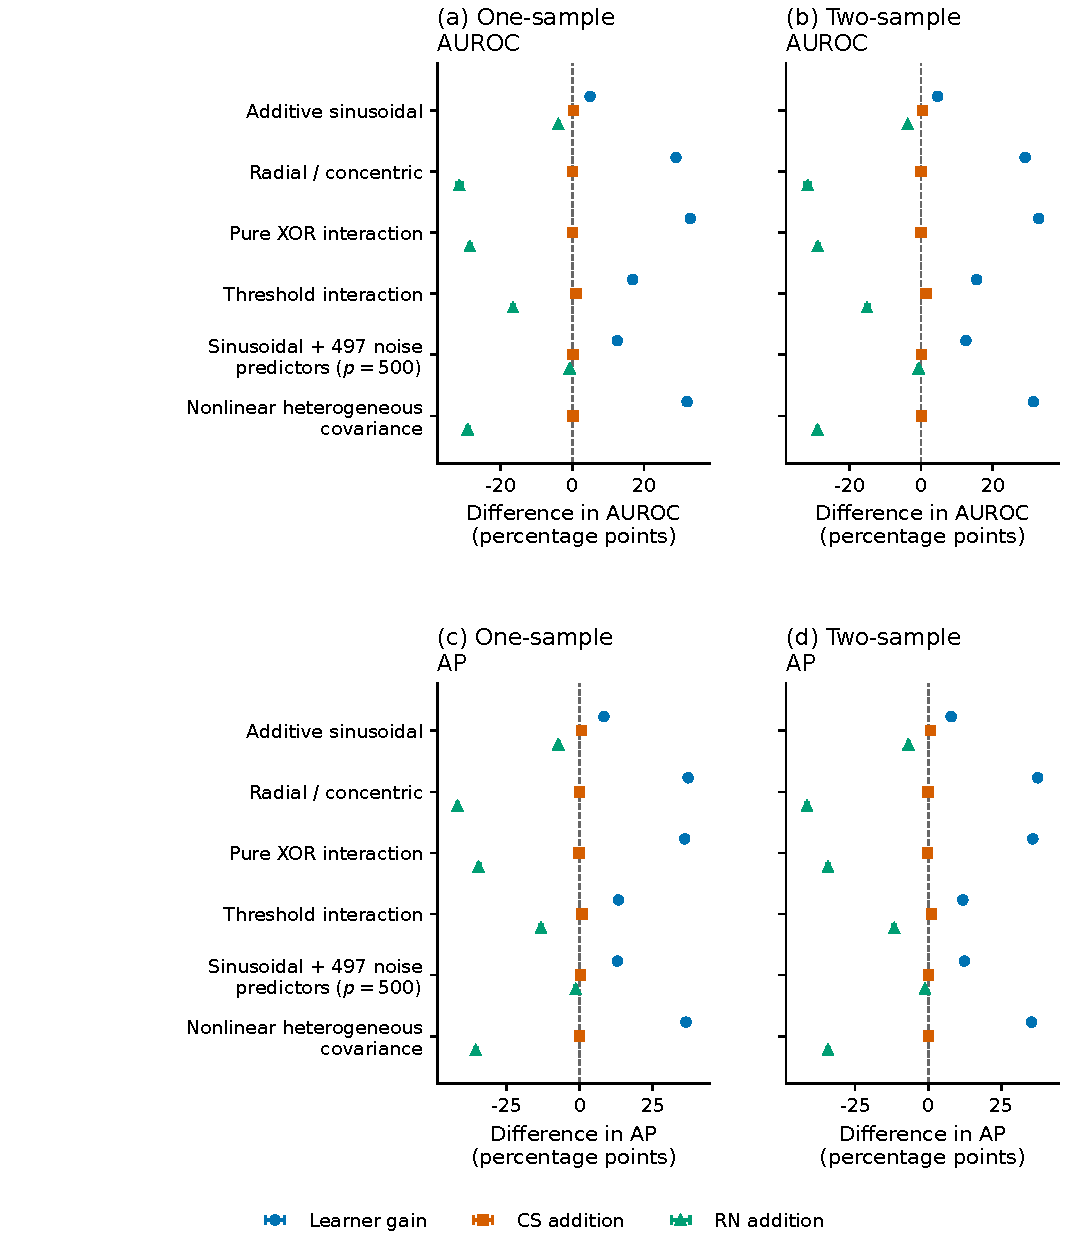
\includegraphics[page=1,width=\textwidth]{mlj_revision/display_package/main/figures/fig_nonlinear_decomposition.pdf}
\caption{Prespecified CatBoost contrasts for each nonlinear DGP: learner gain is naive CatBoost minus logistic probability correction; CS and RN additions hold CatBoost fixed. Points and bars are paired mean differences and 95\% Monte Carlo intervals (mean +/- 1.96 MCSE), in percentage points. Individual DGPs are primary; no DGP average or group maximum is shown. Radial / concentric two-sample RN uses 99 pairs because one final refit is unavailable; all other displayed contrasts use 100. CatBoost learner-versus-strategy decomposition. }
\label{fig:fig-nonlinear-decomposition-page1}
\end{figure*}

